% !TeX encoding = UTF-8
% !TeX program = pdflatex
% !TeX spellcheck = en_US
\documentclass[binding=0.6cm]{sapthesis}
\usepackage{microtype}
\usepackage[english]{babel}
\usepackage[utf8]{inputenc}

%\usepackage{setspace}
%\singlespacing
%\linespread{0.9}
%\usepackage[backend=bibtex,citestyle=authoryear,bibstyle=apa]{biblatex}
\usepackage[backend=biber,style=apa]{biblatex}
\bibliography{bibliography}

%%%% ZAVVE: to add parenthesis to \cite{} command
\newcommand{\mycite}[1]{(\cite{#1})}

\usepackage{hyperref}
\hypersetup{
    %hyperfootnotes=true,			
    %bookmarks=true,			
    %colorlinks=true,
    %linkcolor=red,
    %linktoc=page,
    %anchorcolor=black,
    %citecolor=red,
    %urlcolor=blue,
    pdftitle={Parametrized CF Explanations in Graph Neural Networks},
    pdfauthor={Giammarco D'Alessandro},
    pdfkeywords={thesis, sapienza, roma, university}
 }


\title{Parametrized Counterfactual Explanations for Node Classification in Graph Neural Networks}
\author{Giammarco D'Alessandro}
\IDnumber{1753102}
\course{Corso di laurea magistrale in Engineering in Computer Science - Ingegneria Informatica}
\courseorganizer{Facoltà di Ingengneria dell'Informazione, Informatica e Statistica}
\AcademicYear{2022/2023}
\advisor{Prof. Fabrizio Silvestri}
\coadvisor{Prof. Simone Scardapane}
%\examdate{... November 2023}
\authoremail{dalessandro.1753102@studenti.uniroma1.it}
\copyyear{2023}
%\thesistype{Master thesis}

\begin{document}

\frontmatter
\maketitle
\dedication{Dedicato a\\ Fulmine di Pegasus}

\begin{abstract}
Given the increasing popularity of Graph Neural Networks (GNNs) in real-world applications such as computational biology, natural language processing (NLP), and computer security, etc...; and the \textit{black-box} nature of such models, several methods have been developed for explaining their predictions. One recent approach to address this problem is counterfactual reasoning, where the goal of an explainer algorithm is to induce a change in the GNN prediction by minimal perturbation of the input structure. 

%Existing methods for interpreting predictions from GNNs have primarily focused on generating subgraphs that are especially relevant for a particular prediction. However, such methods are not counterfactual (CF) in nature: given a prediction, we want to understand how the prediction can be changed in order to achieve an alternative outcome. In this work, we propose a method for generating CF explanations for GNNs: the minimal perturbation to the input (graph) data such that the prediction changes. Using only edge deletions, we find that our method, CF-GNNExplainer, can generate CF explanations for the majority of instances across three widely used datasets for GNN explanations, while removing less than 3 edges on average, with at least 94\% accuracy. This indicates that CF-GNNExplainer primarily removes edges that are crucial for the original predictions, resulting in minimal CF explanations.

%Graph neural networks (GNNs) find applications in various domains such as computational biology, natural language processing, and computer security. Owing to their popularity, there is an increasing need to explain GNN predictions since GNNs are black-box machine learning models. One way to address this is counterfactual reasoning where the objective is to change the GNN prediction by minimal changes in the input graph. Existing methods for counterfactual explanation of GNNs are limited to instance-specific local reasoning. This approach has two major limitations of not being able to offer global recourse policies and overloading human cognitive ability with too much information. In this work, we study the global explainability of GNNs through global counterfactual reasoning. Specifically, we want to find a small set of representative counterfactual graphs that explains all input graphs. Towards this goal, we propose GCFExplainer, a novel algorithm powered by vertexreinforced random walks on an edit map of graphs with a greedy summary. Extensive experiments on real graph datasets show that the global explanation from GCFExplainer provides important high-level insights of the model behavior and achieves a 46.9% gain in recourse coverage and a 9.5% reduction in recourse cost
\end{abstract}

\tableofcontents
\mainmatter

%%%%%%%%%%%%%%%%%%%%%%%%% CHAP.1 : Introduction 
\chapter{Introduction}
\label{chap:1} 
In recent years, Graph Neural Networks (GNNs) have emerged as a powerful tool for analyzing complex relational data represented in the form of graphs. Graphs are pervasive in various domains, including social networks, biological systems, transportation networks, and recommendation systems. The ability of GNNs to model and understand these graph structures has led to significant advancements in tasks such as node classification, link prediction, and community detection.

Node classification, a fundamental task in graph analysis, involves predicting labels or categories for nodes in a graph based on their structural and attribute information. Despite the remarkable success of GNNs in node classification, interpreting their decisions remains a challenge. Understanding why a GNN predicts a specific label for a node is crucial for building trust, improving model robustness, and gaining insights into the underlying data.

One promising approach to address the interpretability challenge in GNNs is the integration of counterfactual explanations. Counterfactual explanations provide meaningful insights into model predictions by identifying what changes in the input features would lead to a different prediction. In the context of node classification, counterfactual explanations can elucidate the necessary alterations to the node's attributes or connections that would result in a different predicted label.

This thesis focuses on the incorporation of counterfactual explanations to enhance interpretability in GNNs for node classification. We explore how these explanations can shed light on the decision-making process of GNNs and provide actionable insights for stakeholders. The objective is to bridge the gap between predictive accuracy and model interpretability, facilitating the deployment of GNNs in real-world applications where transparency and trustworthiness are paramount.

In this introductory chapter, we present an overview of the research problem, define the research objectives, outline the scope and contributions of this thesis, and provide a brief outline of the subsequent chapters. Additionally, we discuss the significance of counterfactual explanations in the context of GNNs and node classification, setting the stage for the subsequent chapters that delve deeper into this research domain.


%%%%%%%%%%%%%%%%%%%%%%%%% CHAP.2 : Introduction
\chapter{Background}
\label{chap:2}
Background in generale, intro al background

\section{Graph Neural Networks}
\label{sec:gnns}
Graph Neural Networks (GNNs, \cite{gnnModel2009}) represent a revolutionary paradigm in the field of machine learning, particularly suited for analyzing and extracting insights from complex structured data, such as graphs. Traditional neural networks excel at processing signals like images, speech, videos or sequences in which there is an underlying Euclidean structure, but they struggle with non-Euclidean data, like graphs. Such kinds of data implies that there are no such familiar properties as global parameterization, common system of coordinates, vector space structure, or shift-invariance. Consequently, basic operations like convolution that are taken for granted in the Euclidean case are even not well defined on non-Euclidean domains \mycite{Bronstein_2017}. 

Graph Neural Networks, on the other hand, have emerged as a powerful tool for handling these intricate data structures by incorporating graph-related properties. Recent developments have increased their capabilities and expressive power. Practical applications have become popular in a really wide spectrum of different areas such as drug discovery \mycite{doi:10.1021/acs.jmedchem.9b00959}, physics simulations \mycite{sanchezgonzalez2020learning}, fake news detection \mycite{monti2019fake}, recommendation systems \mycite{eksombatchai2017pixie} and many others \mycite{hamilton2020graph}.

In essence, GNNs are a class of deep learning models designed to operate on graphs, capturing both the node-level and the edge-level information within a graph. They are engineered to learn meaningful representations of nodes and edges by leveraging the graph's topology and associated features. These representations can be exploited in performing various tasks, such as node classification, link prediction, community detection, and graph generation. More generally GNNs have shown remarkable performance in domains where relationships and interactions between entities are crucial for understanding system dynamics and making informed predictions.

This introduction will delve deeper into the foundations, architectures, and applications of Graph Neural Networks, providing a comprehensive understanding of this cutting-edge approach to processing complex relational data. First it will go through some basics of graph theory and it will analyze how these concepts can be used to model real world scenarios, and how neural networks  can exploit the information encoded in such models. Last it will added a brief presentation of different types of GNNs and their peculiarities.

\subsection{From graphs to Graph Neural Networks}
\label{sec:bg.graph_base}
The theory of graphs (also graph theory) can be traced back at least to the illustrious swiss mathematician Leonhard Euler, who in a 1736 paper \mycite{gazette_1987} solved a puzzle about an optimal tour of the town of Königsberg. Some more developments were made in the $19th$ century, the very term "graph" was introduced in this period by Sylvester in a paper published in 1878 in Nature \mycite{Sylvester1878ChemistryAA}, where he draws an analogy between "quantic invariants" and "co-variants" of algebra and molecular diagrams. The field straight-up exploded during the $20th$ century, the first textbook on graph theory was published in 1936 by Dénes Kőnig, followed by many others \mycite{tutte2001graph}; currently graphs are one of the principal objects of study in discrete mathematics. Graphs, in the realm of mathematics and computer science, are powerful mathematical abstractions used to model relationships between entities. In its basic type, a simple graph G can be defined as the couple:
\begin{equation}
    \label{eq:bg.graph_def}
    G = (V,E)
\end{equation}
where $V = \{v_1,v_2,...,v_N\}$ is the set of \textit{vertices} or \textit{nodes}, the entities ($N = |V|$), and $E = \{(v_i,v_j) | v_i,v_j \in V; i \ne j\}$ is the set of \textit{edges}, also called links, modeling the relationship between two entities. A basic distinction is made between \textit{undirected} graphs, where edges link two vertices symmetrically, i.e. there is no difference between the edges $(v_i,v_j)$ and $(v_j,v_i)$; and \textit{directed} graphs, where edges link two vertices asymmetrically, thus $(v_i,v_j)$ and $(v_j,v_i)$ would be two separated edges \mycite{cormen2022introduction}. Moreover two other categorization are generally made: considering the types of its components and their behavior  over time. 
A graph can be \textit{homogeneous}, when nodes and edges of the graph have all the same type; or \textit{heterogeneous} when nodes and edges are associated with different types. More specifically, in a heterogeneous graph $(V, E, \phi, \psi)$, each node $v_i$ is associated with a type $\phi(vi)$ and each edge $e_j$ with a type $\psi(ej)$. 
When input features or the topology of the graph vary with time, i.e. the existence of nodes and edges may change at different points in time, the graph is regarded as \textit{dynamic}, otherwise is considered \textit{static}. The time information should be carefully considered in dynamic graphs \mycite{zhou2021graph,wang2021mthetgnn}. Note that these categories are orthogonal, meaning that these properties can be combined in the same graph, e.g. one can deal with a dynamic directed heterogeneous graph.
%%% cyclic/acyclic graph

%%% more detailed examples
One of the typical application of graphs is modeling the relationships inside social networks \mycite{Wu_Lian_Xu_Wu_Chen_2020}, tools to study patterns in collective behaviour of people, institutions and organizations, where the set of social actors can be represented with the nodes of the graph, and their relative interactions are represented by the edges (e.g. the standard example for a social graph would be a “friendship graph”; here, $V$ is again a set of people and $E$ is the set of $(u, v) \in V$ such that $u$ and $v$ are friends). This perspective on social network provides a set of methods for analyzing the structure of whole social entities as well as a variety of theories explaining the dynamics and patterns observed in these structures \mycite{wasserman_faust_1994}. Even though realities such as social networks can be easily seen as graphs and modeled accordingly this data structures are an extremely powerful and general representation of data, many other domains can actually be modeled as graphs, like images and text. Although counterintuitive, one can learn more about the symmetries and structure of images and text by viewing them as graphs. 
Traditionally, we visualize images as rectangular grids with image channels, often representing them as arrays. However, an alternative way could be seeing images as graphs possessing a regular structure, where each pixel is a node connected to each neighboring pixels through an edge. Specifically, each non-border pixel will maintain precisely 8 neighbors, and the information stored at every node could be a 3-dimensional vector signifying the RGB value of the corresponding pixel. Also text can be easily converted into a graph format by assigning numerical indices to individual characters, words, or tokens, thus creating a sequence of these indices to represent the text. This process yields a straightforward directed graph, where each word or token is a node connected to the succeeding node through an edge. Of course, this is not usually how text and images are encoded: these graph representations are redundant since all images and all text will have very regular structures. In practice, images have a banded structure in their adjacency matrix because all nodes (pixels) are connected in a grid; and the adjacency matrix for text is just a diagonal line, because each word only connects to the prior word, and to the next one, but those trivial examples are supposed to serve as an intuition of how flexible graphs are and how wide can thus be the range of their applications \mycite{distilPub-sanchez-lengeling2021a}.

%%% graph representation, adjacency list/mat ecc...
\subsubsection{Graph representation}
Before going into the details of machine learning applied to graphs, we propose here an introduction on how to represent graphs, their components and the relative features. This problem is crucial to encode real world information into graph models and to be able to exploit the complete potentiality of such abstractions in real world applications. Machine learning models typically take rectangular or grid-like arrays as input, more generally we talk about tensors. In mathematics, a tensor is an algebraic object that describes a multilinear relationship between sets of algebraic objects related to a vector space. Tensors may map between different objects such as vectors, scalars, and even other tensors \mycite{Vasilescu2009AM}. In machine learning, tensors have a broader definition and usually refers also to multidimensional arrays, often called informally "data tensors". The rationale behind this representation is that data stored in such a format can be readily fed into any artificial intelligence model based on neural networks, thereby opening up the possibility of analyzing them through a diverse range of algorithms and models. So, it’s not immediately intuitive how to represent graph structured data in a format that is compatible with deep learning.

Graphs can have up to four types of elements that can be potentially useful to perform machine learning tasks: nodes, edges and connectivity. A solution to represent the first two is relatively straightforward. The most common choice to represent nodes is to assign to each node $v$ an index $i$ (e.g. an integer) as an identifier, and a $d$-dimensional vector to encode the node features, so that, in general, we will have a node feature matrix $X$ of dimension ${N \times d}$ grouping all node data. For what concerns edges we can simply follow the definition (Sec.\ref{sec:bg.graph_base}) identifying each edge $e$ by the couple of nodes it connects in the graph (e.g. if edge $e$ connect nodes $i$ and $j$, we have $e = (v_i,v_j)$) and follow the same idea, if necessary, to encode edge features (in this case the edge feature matrix will have dimension $M \times d$, being $M$ the number of edges) \mycite{cormen2022introduction}. However, representing a graph’s connectivity is more complicated. Several data structures have been proposed to tackle this problem, among them three have resulted to be the most efficient and thus the most used in practice: adjacency matrix, incidence matrix and adjacency list.

The \textit{adjacency matrix} is a two-dimensional tensor ($N \times N$, being $N$ the number of nodes), in which the rows represent source vertices and columns represent destination vertices. Data on edges and vertices must be stored externally. Only the cost for one edge can be stored between each pair of vertices. We note that any two vertices connected by an edges are called adjacent, thus the term \textit{adjacency}. The \textit{incidence matrix} is a two-dimensional tensor ($N \times M$, being $M$ the number of edges), in which the rows represent the vertices and columns represent the edges, so that the entries indicate the incidence relation between the vertex at a row and edge at a column (an edge $e$ is said to be incident to a node $v$, if $e$ is connected to $v$). \textit{Adjacency lists} can be of two types. In one case nodes can be stored as records or objects, and every vertex stores the list of its adjacent vertices. This data structure allows the storage of additional data on the vertices, and even additional data on edges can be stored if they are also stored as objects, in which case each vertex stores its incident edges and each edge stores its incident vertices. The second case is the most common format of \textit{adjacency list}, where all edges are stored together in one single list, which loses the explicit information of the vertices adjacent to a particular node, gaining on efficiency on space usage \mycite{cormen2022introduction}.  

Perhaps, since it can be easily tensorisable the most obvious choice would be to use an adjacency matrix to represent a graph for machine learning purposes. Yet, this particular representation comes with certain limitations. As illustrated by the example dataset table, the quantity of nodes within a real world graph can reach millions, with a highly fluctuating number of edges per node. Consequently, this frequently results in adjacency matrices with significant sparsity, rendering them highly inefficient in terms of space usage. Another big issue is that there can be many adjacency matrices encoding the same connectivity relations (i.e. the same graph), and there could be no guarantee that these different matrices would produce the same result in a deep neural network, that is to say, they are not permutation invariant. The permutation invariance property is a fundamental inductive bias of graph-structured data, resulting in the fact that for a graph with $N$ nodes, there are up to $N!$ different adjacency matrices that are equivalent representations of the same graph. Learning permutation invariant operations is an indipendent area of recent research, we refer the reader to \mycite{mena2018learning,murphy2019janossy} for further details.

There are now dozens (if not hundreds) textbooks available on the subject (\cite{griffin2023applied,cormen2022introduction,diestel2017graph,bondy2011graph,berge1976graphs}; only to cite few relevant ones); we refer the reader to the mentioned books to delve further into the details of all aspects of graph theory given that such a discussion deviates from the main purpose of this background introduction, which is to show the importance of graphs in mathematics, computational sciences and various fields, and why recently a great interest in applying deep learning to these concepts arose. 

%%% ML sui grafi
\subsection{Deep Learning on graphs}
Deep learning is part of a broader family of machine learning (ML) methods, mainly based on extracting patterns from raw data using Artificial Neural Networks (ANNs) and representation learning. The adjective "deep" in deep learning refers to learning complicated concepts by building them from simpler ones in a hierarchical or multi-layer manner \mycite{LeCun2015DeepL}. Artificial neural networks are popular realizations of such deep multi-layer hierarchies. In the past few years, the growing computational power of modern GPU-based computers and the availability of large training datasets have allowed successfully training neural networks with many layers and degrees of freedom \mycite{Bronstein_2017}.

Geometric deep learning is an umbrella term for emerging techniques attempting to generalize (structured) deep neural models to non-Euclidean domains such as graphs and manifolds. As a unique non-Euclidean data structure for machine learning, graph analysis focuses on tasks such as graph classification, node classification, link prediction, and clustering. Graph Neural Networks (GNNs) represent a category of deep learning techniques tailored for processing graph data. Their impressive performance has propelled these deep learning models to the forefront of widely utilized methods in graph analysis today. The first motivation of GNNs is rooted in the long-standing history of neural networks for graphs. In the nineties, Recursive Neural Networks are first utilized on directed acyclic graphs (\cite{Sperduti1997,Frasconi1998}). Afterwards, Recurrent Neural Networks and Feedforward Neural Networks are introduced into this literature respectively in (\cite{gnnModel2009}) and (\cite{Micheli2009}) to tackle cycles. Although being successful, the universal idea behind these methods is building state transition systems on graphs and iterate until convergence, which constrained the extendability and representation ability. Recent advancement of deep neural networks, especially convolutional neural networks (CNNs) result in the rediscovery of GNNs. 

%%% representation learning 
Representation Learning, which is the task of learning representations for complex structured data, is quite challenging with non-euclidean ones. In the last decade, many successful models have been developed for certain kinds of structured data, including data defined on a discretized Euclidean domain. For instance, sequential data, such as text or videos, can be modelled via recurrent neural networks \mycite{TEAlab2018334}, which can capture sequential information, yielding efficient representations as measured on machine translation and speech recognition tasks. Another example are Convolutional Neural Networks (CNNs)\mycite{Lecun1998cnn} have been successfully applied to tackle problems such as image classification (\cite{venkatesan2017convolutional}), semantic segmentation (\cite{jégou2017layers}) or machine translation (\cite{gehring2017convolutional}), where the underlying data representation has a grid-like structure. These architectures efficiently reuse their local filters, with learnable parameters, by applying them to all the input positions \mycite{LeCun2015DeepL}. However these major successes have been restricted to particular types of data that have a simple relational structure (e.g. sequential data, or data following regular patterns), many interesting tasks involve data that can not be represented in a grid-like structure and that instead lies in an irregular domain. This is the case of a large number of systems across various areas including natural science (physical systems (\cite{pmlr-v80-sanchez-gonzalez18a}), social science (social networks as in the example in Sec.\ref{sec:gnns}), protein-protein interaction networks (\cite{nips2017_PPI}), knowledge graphs (\cite{ijcai2017p250}) and many other research areas (\cite{nips2017_combOpt}), to name a few. Such data can usually be represented in the form of graphs \mycite{veličković2018gat}.

%Machine learning with graphs blends the line between this distinction because of two key differences in approaching the problem.

\subsection{GNNs}
Graph Neural Networks (GNNs) have been introduced in \mycite{Gori2005graphDomain,gnnModel2009} as a generalization of recursive neural networks that can directly deal with a more general class of graphs, e.g. cyclic, directed and undirected graphs. The fundamental principle behind GNNs is to produce representations of graph (and/or its components) that can be used in downstream tasks such as graph or node classification.

This first step of GNN design, usually called Graph Representation Learning (GRL) aim at learning low-dimensional continuous vector representations for graph-structured data, also called embeddings. Broadly speaking, GRL can be divided into two classes of learning problems, unsupervised and supervised (or semi-supervised) GRL. The first family aims at learning low-dimensional Euclidean representations that preserve the structure of an input graph. The second family also learns low-dimensional Euclidean representations but for a specific downstream prediction task such as node or graph classification. Different from the unsupervised setting where inputs are usually graph structures, in supervised settings inputs are usually composed of different signals defined on graphs, commonly known as node or edge features.

\begin{figure}
    \label{fig:bg.graph_repr}
    \centering
    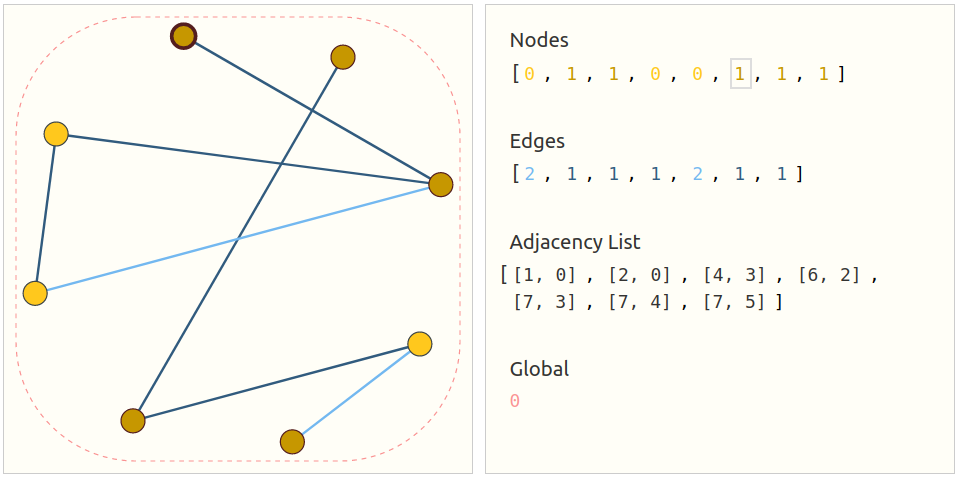
\includegraphics[width=\textwidth]{imgs/background/graph-repr.png}   
    \caption{the dataset format, one json row}
\end{figure}

It should be noted that the figure uses scalar values per node/edge/global, but most practical tensor representations have vectors per graph attribute. Instead of a node tensor of size [nnodes] we will be dealing with node tensors of size [nnodes,nodedim]. Same for the other graph attributes.


GNNs consist of an iterative process, which propagates the node states until equilibrium; followed by a neural network, which produces an output for each node based on its state. This idea was adopted and improved by Li et al. (2016), which propose to use gated recurrent units (Cho et al., 2014) in the propagation step.

Having introduced the basic concepts around graphs, to better better comprehend their success we present an overview of the principal tasks that can be performed through graph representation. There are three general types of prediction tasks on graphs: graph-level, node-level, and edge-level.

In a graph-level task, our goal is to predict the property of an entire graph. For example, for a molecule represented as a graph, we might want to predict what the molecule smells like, or whether it will bind to a receptor implicated in a disease. This is analogous to image classification problems with MNIST and CIFAR,  where we want to associate a label to an entire image. With text, a similar problem is sentiment analysis where we want to identify the mood  r emotion of an entire sentence at once. For a node-level task, we predict some property for each node in a graph. 

For an edge-level task, we want to predict the property or presence of edges in a graph.

For the three levels of prediction problems described above (graph-level, node-level, and edge-level), we will show that all of the following problems can be solved with a single model class, the GNN. But first, let’s take a tour through the three classes of graph prediction problems in more detail, and provide concrete examples of each.


\subsection{Pooling and message passing}
\subsection{GNNs architectures}

\section{Explainability - XAI}
\label{sec:xai}
Explainable Artificial Intelligence (XAI) stands at the forefront of the evolving field of artificial intelligence (AI) and seeks to bridge the gap between advanced AI models and human comprehension. As AI systems become increasingly sophisticated and pervasive in our lives, understanding their decision-making processes and outcomes is crucial for fostering trust, transparency, and usability. XAI aims to unravel the 'black box' nature of complex AI algorithms, providing insights into how these models arrive at specific conclusions or predictions.

In this introduction, we will delve into the core concepts and principles of Explainable AI, exploring its significance, methodologies, and applications. Understanding XAI not only empowers AI practitioners to design more transparent and accountable models but also enables users, stakeholders, and decision-makers to make informed judgments and establish a harmonious coexistence with AI technologies.

\subsection{Explainability vs Interpretability}
\subsection{Explainability in GNNs}
Lallero \mycite{ying2019gnnexplainer}
\subsection{Counterfactual reasoning}


%%%%%%%%%%%%%%%%%%%%%%%%% CHAP.3 : My method
\chapter{Parametrized Counterfactual Explainations for Node Classification in Graph Neural Networks}
\label{chap:3}
\section{Related works}
\label{sec:gcf}
Despite the impressive success of GNNs on predictive tasks, GNNs are black-box machine learning models. It is non-trivial to explain or reason why a particular prediction is made by a GNN. Explainability of a prediction model is important to understand its shortcomings and identify areas for improvement. In addition, the ability to explain a model is critical towards making it trustworthy. Owing to this limitation of GNNs, there has been significant efforts in recent times towards explanation approaches. Existing work on explaining GNN predictions can be categorized mainly in two directions: 1) factual reasoning [20, 40, 46, 47], and 2) counterfactual reasoning [1, 2, 19, 36]. Generally speaking, the methods in the first category aim to find an important subgraph that correlates most with the underlying GNN prediction. In contrast, the methods with counterfactual reasoning attempt to identify the smallest amount of perturbation on the input graph that changes the GNN’s prediction, for example, removal/addition of edges or nodes. Compared to factual reasoning, counterfactual explainers have the additional advantage of providing the means for recourse [39].

\subsection{Global e local CF}

\section{Problem formal definition}
\label{sec:form-def}
\section{Proposed Approach}
\label{sec:cfpg}
\subsection{Discrete latent structures}
Lallero \mycite{niculae2023discrete}


%%%%%%%%%%%%%%%%%%%%%%%%% CHAP.4 : Experiments
\chapter{Experimental results}
\label{chap:4}

\section{Synthetic datasets}
\label{sec:syns}

\section{Preprocessing}
\label{sec:prepro}
Property of the European Southern Observatory...

\section{countefactual metrics}
\label{sec:metrics}
The \textit{Multi-Object Optical and Near-infrared Spectrograph} is a future generation MOS instrument for the VLT. 

\section{Results}
\label{sec:res}


%%%%%%%%%%%%%%%%%%%%%%%%% CHAP.5 : Conclusions
\chapter{Conclusions}
\label{chap:5} 
The grasping power of the mirror..





\backmatter
\cleardoublepage % blank page after each chapter

%%%%%%%%%%%%%%%%%%%%%%%%% bibliography
\phantomsection % Give this command only if hyperref is loaded
\addcontentsline{toc}{chapter}{\bibname}
% Here put the code for the bibliography. You can use BibTeX or
% the BibLaTeX package or the simple environment thebibliography.
\printbibheading
\printbibliography[type=article,heading=subbibliography,title={Articles}]
\printbibliography[type=inbook,heading=subbibliography,title={Inproceedings}]
\printbibliography[type=book,heading=subbibliography,title={Books}]
\printbibliography[type=misc,heading=subbibliography,title={Miscellaneous}]

\end{document}